\section{Shared Response Directions and Their Effect on Commands}
\label{sec:structured}
This section follows the first two links in $\pi_{0.5}$: what a perturbation changes in the features, and whether undoing that change moves the commands.

\subsection{Different Perturbations Change Features along Shared Directions}
\label{sec:shared}
Do different perturbations change the features in a common way? At each recorded layer we fit 16 directions to the responses by principal component analysis (PCA), with the policy frozen, and call them the \emph{shared directions}. PCA finds the directions along which the fitted responses vary most, so a fair test must use responses it has not seen. Each fit therefore leaves out both the tasks and the perturbation family on which it is tested: directions tested on Camera responses, for example, are fitted without any Camera response and without the test tasks. Tasks that share a clean scene are left out together.

We then ask how much of an unseen response these directions retain. Responses are taken at the first generation step ($j=0$) of the first query, where the clean and perturbed runs share the same noisy plan and differ only in the image. With $\Delta H_i$ the response for the $i$-th planned action, $\mu_i$ its mean over the fitting data, and $B\in\mathbb R^{1024\times16}$ the directions, the reconstruction is
\begin{equation}
\widehat{\Delta H}_i=\mu_i+(\Delta H_i-\mu_i)BB^\top.
\label{eq:p08-reconstruction}
\end{equation}
We report the share of the response energy, the squared magnitude of $\Delta H-\mu$, that the reconstruction retains (Supplement, Sec.~S3). Two controls also use 16 directions: \emph{clean-feature directions}, fitted to clean features, which test whether responses simply follow ordinary feature variation, and \emph{random directions}, which show what chance gives.

The shared directions retain 36.5--83.6\% of the response energy, most at L1 and least at L18 in every family. Clean-feature directions retain at most 10.2\%, and random directions about 1.6\% (Fig.~\ref{fig:token-structure}a). Measured against the raw response energy, without subtracting $\mu$, the same reconstruction retains 16.3--75.0\% on the full 40-task panel (Supplement, Table~S5). No fit saw the tasks or the family on which it is tested, so the match cannot come from fitting to the test data: different perturbations change the features along common directions. The result holds for other numbers of directions, in $\pi_0$, and at later observations of an episode (Supplement, Secs.~S3, S14, and~S8.1).

\begin{figure*}[t]
\centering
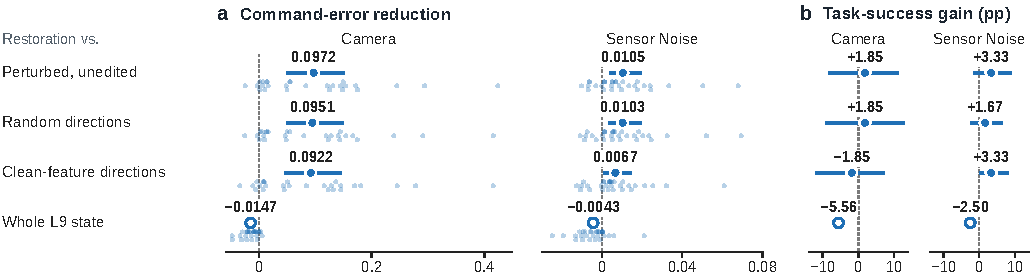
\includegraphics[width=\textwidth]{revised_figures/figure4_restoration_v3.pdf}
\caption{\textbf{Restoration against the unedited perturbed run, the two controls, and replacing the whole L9 state.}
Each row compares restoration with another run of the same cases (31 held-out tasks; Camera: 27 tasks, 96 cases; Sensor Noise: 30 tasks, 120 cases). Positive values favor restoration; negative values favor the other run, as for the whole L9 state on both measures. (a) Command error of the other run minus that of restoration: mean with simultaneous 95\% interval; small dots are tasks. Restoration lowers the command error of the unedited run in 25 of 27 and 24 of 30 tasks, and reduces it more than both controls, which also write less (edit size, Table~\ref{tab:restoration}). (b) Primary endpoint: success of restoration minus that of the other run, in percentage points, with intervals as in (a). The random-direction run under Camera and the clean-feature run under Sensor Noise succeed as often as the unedited run (Table~\ref{tab:restoration}), so their rows repeat its means. The whole-L9 run was not among the six prespecified comparisons, so it has no interval (open marks). Axes differ between families.}
\label{fig:native-restoration}
\end{figure*}


\textbf{From responses to commands.}\label{sec:layers} Do the coordinates along the shared directions also tell how the commands change? A linear readout of the 16 coordinates predicts the change in the first five commands best at L18, the last block before the output, and poorly at L1 and L9 (Fig.~\ref{fig:token-structure}b; Supplement, Secs.~S3.4 and~S13). The layer that retains the most response is thus not the layer from which the commands are best read. A readout, moreover, tests only what can be read from these coordinates; restoring them inside the policy tests what they change. We therefore test the directions by intervening.

\subsection{Restoring the Shared Directions Reduces Command Error}
\label{sec:restoration}
If the shared directions matter for the commands, undoing the perturbation along them should move the commands back toward those of the clean run. \emph{Restoration} does this at L9. At every generation step of every query, it computes what the L9 state would be under a clean observation of the same physical state, and copies the clean values along the 16 shared directions into the perturbed run (Fig.~\ref{fig:model-measurement}c). With $H^c$ and $H^p$ the clean and perturbed L9 states,
\begin{equation}
H'=H^p-(H^p-H^c)BB^\top.
\label{eq:coordinate-restoration}
\end{equation}
Everything else stays perturbed: the rest of the L9 state, and the image that blocks 10--18 still read. This is activation patching~\cite{meng2022locating} restricted to the shared directions. It needs a clean observation of the same state, so it is a controlled test and not a method one could deploy. We fixed L9, the middle layer, in advance, as a compromise between L1, which retains the most response, and L18, which predicts commands best.

\begin{table}[t]
\centering\small
\setlength{\tabcolsep}{2.6pt}
\begin{tabular}{@{}lrrrrrr@{}}
\toprule
 & \multicolumn{3}{c}{Camera} & \multicolumn{3}{c}{Sensor Noise}\\
\cmidrule(lr){2-4}\cmidrule(l){5-7}
Run & error & succ. & edit & error & succ. & edit\\
\midrule
Perturbed, unedited & 0.409 & 73.15 & -- & 0.209 & 83.33 & --\\
Random directions & 0.407 & 73.15 & 9.7 & 0.209 & 85.00 & 9.6\\
Clean-feature directions & 0.404 & 76.85 & 7.8 & 0.205 & 83.33 & 7.7\\
Restoration & 0.312 & 75.00 & 46.2 & 0.199 & 86.67 & 51.5\\
Whole L9 state & 0.297 & 80.56 & 74.2 & 0.194 & 89.17 & 72.8\\
Clean & 0 & 98.15 & -- & 0 & 97.50 & --\\
\bottomrule
\end{tabular}
\caption{\textbf{The six runs of the restoration test.} Command error (distance of the first five commands from those of the clean run), task success (\%), and edit size (summed change written into the L9 state over an episode, in thousands), averaged with equal weight per task over 96 Camera and 120 Sensor Noise cases. Intervals for the comparisons: Figs.~\ref{fig:teaser}b and~\ref{fig:native-restoration}; Supplement, Tables~S31--S33.}
\label{tab:restoration}
\end{table}


We test restoration on 216 cases (96 Camera, 120 Sensor Noise) from 31 tasks, none of them among the nine used to develop it. Each case is run six times from the same start state with the same policy noise (Table~\ref{tab:restoration}). Besides the clean and the perturbed run, one run applies restoration; two controls restore 16 clean-feature or 16 random directions instead, to show whether any 16 directions would do; and a last run replaces the whole L9 state, to show the most that restoring this layer can do. Task success is the primary endpoint, fixed in advance. The second endpoint is the \emph{command error}: the distance between a run's first five commands and those of the clean run. Directions are again fitted without the test tasks and family (Supplement, Sec.~S12).

\textbf{Command error falls.} Restoration lowers the command error by 24\% for Camera (0.409 to 0.312) and by 5\% for Sensor Noise (0.209 to 0.199), while the two controls leave it almost unchanged (Table~\ref{tab:restoration}; Figs.~\ref{fig:teaser}b and~\ref{fig:native-restoration}a). The error falls in 25 of 27 Camera tasks and 24 of 30 Sensor Noise tasks, and the intervals for all comparisons, with the unedited run and with both controls, exclude zero (Supplement, Sec.~S12.4). The shared directions at L9 therefore carry part of the perturbation's effect on the commands.

\textbf{The shared directions do most of what this layer can do.} Replacing the whole L9 state removes 27\% and 7\% of the command error; the rest enters through the later blocks, which still read the perturbed image. The 16 shared directions, out of 1024 channels, reach 86.9\% and 70.7\% of that (Supplement, Tables~S25--S26).

\textbf{Controls and edit size.} Restoration changes the L9 state five to seven times as much as the two controls (edit size in Table~\ref{tab:restoration}), because more of a clean--perturbed difference lies along directions fitted to such differences. Three comparisons take edit size into account. Per unit of edit, restoration removes 1.4 times as much command error as replacing the whole L9 state under Camera, and as much under Sensor Noise. With edit size matched in development, it brings the first five planned commands closer to the clean ones than clean-feature directions do under Camera, but not under Sensor Noise (Supplement, Sec.~S12.5). And a second test, which needs no clean observation, uses controls of matched size: on original LIBERO (6,048 planned rollouts), removing the L9 components along the shared directions lowers the response at L18 by 8.8\% and 7.6\% under a camera and a lighting change, against at most 0.3\% for random directions (Supplement, Sec.~S11).

\textbf{Task success is also higher.} After restoration, success is higher by 1.85 points for Camera and by 3.33 for Sensor Noise (Table~\ref{tab:restoration}; simultaneous 95\% intervals $[-8.33,11.11]$ and $[-1.67,9.17]$, Fig.~\ref{fig:native-restoration}b; Supplement, Table~S24). Replacing the whole L9 state raises success by 7.41 and 5.83 points (post hoc pointwise intervals $[0.93,14.81]$ and $[0.00,12.50]$; Supplement, Sec.~S12.4): this layer matters for the outcome, and the 16 directions deliver part of that gain.
